% Options for packages loaded elsewhere
\PassOptionsToPackage{unicode}{hyperref}
\PassOptionsToPackage{hyphens}{url}
%
\documentclass[
]{article}
\usepackage{amsmath,amssymb}
\usepackage{iftex}
\ifPDFTeX
  \usepackage[T1]{fontenc}
  \usepackage[utf8]{inputenc}
  \usepackage{textcomp} % provide euro and other symbols
\else % if luatex or xetex
  \usepackage{unicode-math} % this also loads fontspec
  \defaultfontfeatures{Scale=MatchLowercase}
  \defaultfontfeatures[\rmfamily]{Ligatures=TeX,Scale=1}
\fi
\usepackage{lmodern}
\ifPDFTeX\else
  % xetex/luatex font selection
\fi
% Use upquote if available, for straight quotes in verbatim environments
\IfFileExists{upquote.sty}{\usepackage{upquote}}{}
\IfFileExists{microtype.sty}{% use microtype if available
  \usepackage[]{microtype}
  \UseMicrotypeSet[protrusion]{basicmath} % disable protrusion for tt fonts
}{}
\makeatletter
\@ifundefined{KOMAClassName}{% if non-KOMA class
  \IfFileExists{parskip.sty}{%
    \usepackage{parskip}
  }{% else
    \setlength{\parindent}{0pt}
    \setlength{\parskip}{6pt plus 2pt minus 1pt}}
}{% if KOMA class
  \KOMAoptions{parskip=half}}
\makeatother
\usepackage{xcolor}
\usepackage[margin=1in]{geometry}
\usepackage{color}
\usepackage{fancyvrb}
\newcommand{\VerbBar}{|}
\newcommand{\VERB}{\Verb[commandchars=\\\{\}]}
\DefineVerbatimEnvironment{Highlighting}{Verbatim}{commandchars=\\\{\}}
% Add ',fontsize=\small' for more characters per line
\usepackage{framed}
\definecolor{shadecolor}{RGB}{248,248,248}
\newenvironment{Shaded}{\begin{snugshade}}{\end{snugshade}}
\newcommand{\AlertTok}[1]{\textcolor[rgb]{0.94,0.16,0.16}{#1}}
\newcommand{\AnnotationTok}[1]{\textcolor[rgb]{0.56,0.35,0.01}{\textbf{\textit{#1}}}}
\newcommand{\AttributeTok}[1]{\textcolor[rgb]{0.13,0.29,0.53}{#1}}
\newcommand{\BaseNTok}[1]{\textcolor[rgb]{0.00,0.00,0.81}{#1}}
\newcommand{\BuiltInTok}[1]{#1}
\newcommand{\CharTok}[1]{\textcolor[rgb]{0.31,0.60,0.02}{#1}}
\newcommand{\CommentTok}[1]{\textcolor[rgb]{0.56,0.35,0.01}{\textit{#1}}}
\newcommand{\CommentVarTok}[1]{\textcolor[rgb]{0.56,0.35,0.01}{\textbf{\textit{#1}}}}
\newcommand{\ConstantTok}[1]{\textcolor[rgb]{0.56,0.35,0.01}{#1}}
\newcommand{\ControlFlowTok}[1]{\textcolor[rgb]{0.13,0.29,0.53}{\textbf{#1}}}
\newcommand{\DataTypeTok}[1]{\textcolor[rgb]{0.13,0.29,0.53}{#1}}
\newcommand{\DecValTok}[1]{\textcolor[rgb]{0.00,0.00,0.81}{#1}}
\newcommand{\DocumentationTok}[1]{\textcolor[rgb]{0.56,0.35,0.01}{\textbf{\textit{#1}}}}
\newcommand{\ErrorTok}[1]{\textcolor[rgb]{0.64,0.00,0.00}{\textbf{#1}}}
\newcommand{\ExtensionTok}[1]{#1}
\newcommand{\FloatTok}[1]{\textcolor[rgb]{0.00,0.00,0.81}{#1}}
\newcommand{\FunctionTok}[1]{\textcolor[rgb]{0.13,0.29,0.53}{\textbf{#1}}}
\newcommand{\ImportTok}[1]{#1}
\newcommand{\InformationTok}[1]{\textcolor[rgb]{0.56,0.35,0.01}{\textbf{\textit{#1}}}}
\newcommand{\KeywordTok}[1]{\textcolor[rgb]{0.13,0.29,0.53}{\textbf{#1}}}
\newcommand{\NormalTok}[1]{#1}
\newcommand{\OperatorTok}[1]{\textcolor[rgb]{0.81,0.36,0.00}{\textbf{#1}}}
\newcommand{\OtherTok}[1]{\textcolor[rgb]{0.56,0.35,0.01}{#1}}
\newcommand{\PreprocessorTok}[1]{\textcolor[rgb]{0.56,0.35,0.01}{\textit{#1}}}
\newcommand{\RegionMarkerTok}[1]{#1}
\newcommand{\SpecialCharTok}[1]{\textcolor[rgb]{0.81,0.36,0.00}{\textbf{#1}}}
\newcommand{\SpecialStringTok}[1]{\textcolor[rgb]{0.31,0.60,0.02}{#1}}
\newcommand{\StringTok}[1]{\textcolor[rgb]{0.31,0.60,0.02}{#1}}
\newcommand{\VariableTok}[1]{\textcolor[rgb]{0.00,0.00,0.00}{#1}}
\newcommand{\VerbatimStringTok}[1]{\textcolor[rgb]{0.31,0.60,0.02}{#1}}
\newcommand{\WarningTok}[1]{\textcolor[rgb]{0.56,0.35,0.01}{\textbf{\textit{#1}}}}
\usepackage{longtable,booktabs,array}
\usepackage{calc} % for calculating minipage widths
% Correct order of tables after \paragraph or \subparagraph
\usepackage{etoolbox}
\makeatletter
\patchcmd\longtable{\par}{\if@noskipsec\mbox{}\fi\par}{}{}
\makeatother
% Allow footnotes in longtable head/foot
\IfFileExists{footnotehyper.sty}{\usepackage{footnotehyper}}{\usepackage{footnote}}
\makesavenoteenv{longtable}
\usepackage{graphicx}
\makeatletter
\def\maxwidth{\ifdim\Gin@nat@width>\linewidth\linewidth\else\Gin@nat@width\fi}
\def\maxheight{\ifdim\Gin@nat@height>\textheight\textheight\else\Gin@nat@height\fi}
\makeatother
% Scale images if necessary, so that they will not overflow the page
% margins by default, and it is still possible to overwrite the defaults
% using explicit options in \includegraphics[width, height, ...]{}
\setkeys{Gin}{width=\maxwidth,height=\maxheight,keepaspectratio}
% Set default figure placement to htbp
\makeatletter
\def\fps@figure{htbp}
\makeatother
\ifLuaTeX
  \usepackage{luacolor}
  \usepackage[soul]{lua-ul}
\else
  \usepackage{soul}
\fi
\setlength{\emergencystretch}{3em} % prevent overfull lines
\providecommand{\tightlist}{%
  \setlength{\itemsep}{0pt}\setlength{\parskip}{0pt}}
\setcounter{secnumdepth}{5}
\ifLuaTeX
  \usepackage{selnolig}  % disable illegal ligatures
\fi
\usepackage{bookmark}
\IfFileExists{xurl.sty}{\usepackage{xurl}}{} % add URL line breaks if available
\urlstyle{same}
\hypersetup{
  pdftitle={Multiple Linear Regression},
  pdfauthor={Allan Omondi},
  hidelinks,
  pdfcreator={LaTeX via pandoc}}

\title{Multiple Linear Regression}
\author{Allan Omondi}
\date{2025-05-03}

\begin{document}
\maketitle

{
\setcounter{tocdepth}{4}
\tableofcontents
}
\section{Load the Dataset}\label{load-the-dataset}

\begin{Shaded}
\begin{Highlighting}[]
\NormalTok{pacman}\SpecialCharTok{::}\FunctionTok{p\_load}\NormalTok{(}\StringTok{"readr"}\NormalTok{)}

\NormalTok{advertising\_data }\OtherTok{\textless{}{-}} \FunctionTok{read\_csv}\NormalTok{(}\StringTok{"./data/advertising.csv"}\NormalTok{)}
\FunctionTok{head}\NormalTok{(advertising\_data)}
\end{Highlighting}
\end{Shaded}

\begin{verbatim}
## # A tibble: 6 x 4
##   YouTube TikTok Facebook Sales
##     <dbl>  <dbl>    <dbl> <dbl>
## 1    1200    800     1000  95.3
## 2    1500    900     1100 101. 
## 3    1300    850     1050  99.5
## 4    1600    950     1150 107. 
## 5    1100    780      980  93.0
## 6    1700   1000     1200 108.
\end{verbatim}

\section{Initial EDA}\label{initial-eda}

\ul{\textbf{View the Dimensions}}

The number of observations and the number of variables.

\begin{Shaded}
\begin{Highlighting}[]
\FunctionTok{dim}\NormalTok{(advertising\_data)}
\end{Highlighting}
\end{Shaded}

\begin{verbatim}
## [1] 10  4
\end{verbatim}

\ul{\textbf{View the Data Types}}

\begin{Shaded}
\begin{Highlighting}[]
\FunctionTok{sapply}\NormalTok{(advertising\_data, class)}
\end{Highlighting}
\end{Shaded}

\begin{verbatim}
##   YouTube    TikTok  Facebook     Sales 
## "numeric" "numeric" "numeric" "numeric"
\end{verbatim}

\begin{Shaded}
\begin{Highlighting}[]
\FunctionTok{str}\NormalTok{(advertising\_data)}
\end{Highlighting}
\end{Shaded}

\begin{verbatim}
## spc_tbl_ [10 x 4] (S3: spec_tbl_df/tbl_df/tbl/data.frame)
##  $ YouTube : num [1:10] 1200 1500 1300 1600 1100 1700 1400 1800 1250 1550
##  $ TikTok  : num [1:10] 800 900 850 950 780 1000 880 1020 820 970
##  $ Facebook: num [1:10] 1000 1100 1050 1150 980 1200 1080 1220 1010 1130
##  $ Sales   : num [1:10] 95.3 101.2 99.5 106.8 93 ...
##  - attr(*, "spec")=
##   .. cols(
##   ..   YouTube = col_double(),
##   ..   TikTok = col_double(),
##   ..   Facebook = col_double(),
##   ..   Sales = col_double()
##   .. )
##  - attr(*, "problems")=<externalptr>
\end{verbatim}

\ul{\textbf{Descriptive Statistics}}

\subsection{\texorpdfstring{\ul{\textbf{Measures of
Frequency}}}{Measures of Frequency}}\label{measures-of-frequency}

This is applicable in cases where you have categorical variables, e.g.,
60\% of the observations are male and 40\% are female (2 categories).

\subsection{\texorpdfstring{\ul{\textbf{Measures of Central
Tendency}}}{Measures of Central Tendency}}\label{measures-of-central-tendency}

The median and the mean of each numeric variable:

\begin{Shaded}
\begin{Highlighting}[]
\FunctionTok{summary}\NormalTok{(advertising\_data)}
\end{Highlighting}
\end{Shaded}

\begin{verbatim}
##     YouTube         TikTok          Facebook        Sales       
##  Min.   :1100   Min.   : 780.0   Min.   : 980   Min.   : 93.02  
##  1st Qu.:1262   1st Qu.: 827.5   1st Qu.:1020   1st Qu.: 97.27  
##  Median :1450   Median : 890.0   Median :1090   Median :101.95  
##  Mean   :1440   Mean   : 897.0   Mean   :1092   Mean   :101.93  
##  3rd Qu.:1588   3rd Qu.: 965.0   3rd Qu.:1145   3rd Qu.:106.17  
##  Max.   :1800   Max.   :1020.0   Max.   :1220   Max.   :111.82
\end{verbatim}

\subsection{\texorpdfstring{\ul{\textbf{Measures of
Distribution}}}{Measures of Distribution}}\label{measures-of-distribution}

Measuring the variability in the dataset is important because the amount
of variability determines \textbf{how well you can generalize} results
from the sample to a new observation in the population.

Low variability is ideal because it means that you can better predict
information about the population based on the sample data. High
variability means that the values are less consistent, thus making it
harder to make predictions.

\subsubsection{\texorpdfstring{\textbf{Variance}}{Variance}}\label{variance}

\begin{Shaded}
\begin{Highlighting}[]
\FunctionTok{sapply}\NormalTok{(advertising\_data[,], var)}
\end{Highlighting}
\end{Shaded}

\begin{verbatim}
##     YouTube      TikTok    Facebook       Sales 
## 52111.11111  7267.77778  6951.11111    36.13165
\end{verbatim}

\subsubsection{\texorpdfstring{\textbf{Standard
Deviation}}{Standard Deviation}}\label{standard-deviation}

\begin{Shaded}
\begin{Highlighting}[]
\FunctionTok{sapply}\NormalTok{(advertising\_data[,], sd)}
\end{Highlighting}
\end{Shaded}

\begin{verbatim}
##   YouTube    TikTok  Facebook     Sales 
## 228.27858  85.25126  83.37332   6.01096
\end{verbatim}

\subsubsection{\texorpdfstring{\textbf{Kurtosis}}{Kurtosis}}\label{kurtosis}

The Kurtosis informs us of how often outliers occur in the results.
There are different formulas for calculating kurtosis. Specifying ``type
= 2'' allows us to use the 2nd formula which is the same kurtosis
formula used in other statistical software like SPSS and SAS.

In ``type = 2'' (used in SPSS and SAS):

\begin{enumerate}
\def\labelenumi{\arabic{enumi}.}
\item
  Kurtosis \textless{} 3 implies a low number of outliers
\item
  Kurtosis = 3 implies a medium number of outliers
\item
  Kurtosis \textgreater{} 3 implies a high number of outliers
\end{enumerate}

\begin{Shaded}
\begin{Highlighting}[]
\NormalTok{pacman}\SpecialCharTok{::}\FunctionTok{p\_load}\NormalTok{(}\StringTok{"e1071"}\NormalTok{)}
\FunctionTok{sapply}\NormalTok{(advertising\_data[,],  kurtosis, }\AttributeTok{type =} \DecValTok{2}\NormalTok{)}
\end{Highlighting}
\end{Shaded}

\begin{verbatim}
##    YouTube     TikTok   Facebook      Sales 
## -1.0800892 -1.4726766 -1.1989242 -0.8697324
\end{verbatim}

\subsubsection{\texorpdfstring{\textbf{Skewness}}{Skewness}}\label{skewness}

The skewness is used to identify the asymmetry of the distribution of
results. Similar to kurtosis, there are several ways of computing the
skewness.

Using ``type = 2'' (common in other statistical software like SPSS and
SAS) can be interpreted as:

\begin{enumerate}
\def\labelenumi{\arabic{enumi}.}
\item
  Skewness between -0.4 and 0.4 (inclusive) implies that there is no
  skew in the distribution of results; the distribution of results is
  symmetrical; it is a normal distribution; a Gaussian distribution.
\item
  Skewness above 0.4 implies a positive skew; a right-skewed
  distribution.
\item
  Skewness below -0.4 implies a negative skew; a left-skewed
  distribution.
\end{enumerate}

\begin{Shaded}
\begin{Highlighting}[]
\FunctionTok{sapply}\NormalTok{(advertising\_data[,], skewness, }\AttributeTok{type =} \DecValTok{2}\NormalTok{)}
\end{Highlighting}
\end{Shaded}

\begin{verbatim}
##    YouTube     TikTok   Facebook      Sales 
## 0.08266188 0.09234643 0.19089944 0.10505432
\end{verbatim}

\subsection{\texorpdfstring{\ul{\textbf{Measures of
Relationship}}}{Measures of Relationship}}\label{measures-of-relationship}

\subsubsection{\texorpdfstring{\textbf{Covariance}}{Covariance}}\label{covariance}

Covariance is a statistical measure that indicates the direction of the
linear relationship between two variables. It assesses whether increases
in one variable correspond to increases or decreases in
another.\hspace{0pt}

\begin{itemize}
\item
  \textbf{Positive Covariance:} When one variable increases, the other
  tends to increase as well.
\item
  \textbf{Negative Covariance:} When one variable increases, the other
  tends to decrease.
\item
  \textbf{Zero Covariance:} No linear relationship exists between the
  variables.
\end{itemize}

While covariance indicates the direction of a relationship, it does not
convey the strength or consistency of the relationship. The correlation
coefficient is used to indicate the strength of the relationship.

\begin{Shaded}
\begin{Highlighting}[]
\FunctionTok{cov}\NormalTok{(advertising\_data, }\AttributeTok{method =} \StringTok{"spearman"}\NormalTok{)}
\end{Highlighting}
\end{Shaded}

\begin{verbatim}
##           YouTube   TikTok Facebook    Sales
## YouTube  9.166667 9.055556 9.166667 9.055556
## TikTok   9.055556 9.166667 9.055556 8.944444
## Facebook 9.166667 9.055556 9.166667 9.055556
## Sales    9.055556 8.944444 9.055556 9.166667
\end{verbatim}

\subsubsection{\texorpdfstring{\textbf{Correlation}}{Correlation}}\label{correlation}

A strong correlation between variables enables us to better predict the
value of the dependent variable using the value of the independent
variable. However, a weak correlation between two variables does not
help us to predict the value of the dependent variable from the value of
the independent variable. This is useful only if there is a linear
association between the variables.

We can measure the statistical significance of the correlation using
Spearman's rank correlation \emph{rho}. This shows us if the variables
are significantly monotonically related. A monotonic relationship
between two variables implies that as one variable increases, the other
variable either consistently increases or consistently decreases. The
key characteristic is the preservation of the direction of change,
though the rate of change may vary.

\textbf{Option 1:} Conduct a correlation test between the dependent
variable and each independent variable one at a time.

\begin{Shaded}
\begin{Highlighting}[]
\FunctionTok{cor.test}\NormalTok{(advertising\_data}\SpecialCharTok{$}\NormalTok{Sales, advertising\_data}\SpecialCharTok{$}\NormalTok{YouTube, }\AttributeTok{method =} \StringTok{"spearman"}\NormalTok{)}
\end{Highlighting}
\end{Shaded}

\begin{verbatim}
## 
##  Spearman's rank correlation rho
## 
## data:  advertising_data$Sales and advertising_data$YouTube
## S = 2, p-value < 2.2e-16
## alternative hypothesis: true rho is not equal to 0
## sample estimates:
##       rho 
## 0.9878788
\end{verbatim}

\begin{Shaded}
\begin{Highlighting}[]
\FunctionTok{cor.test}\NormalTok{(advertising\_data}\SpecialCharTok{$}\NormalTok{Sales, advertising\_data}\SpecialCharTok{$}\NormalTok{TikTok, }\AttributeTok{method =} \StringTok{"spearman"}\NormalTok{)}
\end{Highlighting}
\end{Shaded}

\begin{verbatim}
## 
##  Spearman's rank correlation rho
## 
## data:  advertising_data$Sales and advertising_data$TikTok
## S = 4, p-value < 2.2e-16
## alternative hypothesis: true rho is not equal to 0
## sample estimates:
##       rho 
## 0.9757576
\end{verbatim}

\begin{Shaded}
\begin{Highlighting}[]
\FunctionTok{cor.test}\NormalTok{(advertising\_data}\SpecialCharTok{$}\NormalTok{Sales, advertising\_data}\SpecialCharTok{$}\NormalTok{Facebook, }\AttributeTok{method =} \StringTok{"spearman"}\NormalTok{)}
\end{Highlighting}
\end{Shaded}

\begin{verbatim}
## 
##  Spearman's rank correlation rho
## 
## data:  advertising_data$Sales and advertising_data$Facebook
## S = 2, p-value < 2.2e-16
## alternative hypothesis: true rho is not equal to 0
## sample estimates:
##       rho 
## 0.9878788
\end{verbatim}

\textbf{Option 2:} To view the correlation of all variables at the same
time

\begin{Shaded}
\begin{Highlighting}[]
\FunctionTok{cor}\NormalTok{(advertising\_data, }\AttributeTok{method =} \StringTok{"spearman"}\NormalTok{)}
\end{Highlighting}
\end{Shaded}

\begin{verbatim}
##            YouTube    TikTok  Facebook     Sales
## YouTube  1.0000000 0.9878788 1.0000000 0.9878788
## TikTok   0.9878788 1.0000000 0.9878788 0.9757576
## Facebook 1.0000000 0.9878788 1.0000000 0.9878788
## Sales    0.9878788 0.9757576 0.9878788 1.0000000
\end{verbatim}

\subsection{\texorpdfstring{\ul{\textbf{Basic
Visualizations}}}{Basic Visualizations}}\label{basic-visualizations}

\subsubsection{\texorpdfstring{\textbf{Histogram}}{Histogram}}\label{histogram}

\begin{Shaded}
\begin{Highlighting}[]
\FunctionTok{par}\NormalTok{(}\AttributeTok{mfrow =} \FunctionTok{c}\NormalTok{(}\DecValTok{1}\NormalTok{, }\DecValTok{2}\NormalTok{))}
\ControlFlowTok{for}\NormalTok{ (i }\ControlFlowTok{in} \DecValTok{1}\SpecialCharTok{:}\DecValTok{4}\NormalTok{) \{}
  \ControlFlowTok{if}\NormalTok{ (}\FunctionTok{is.numeric}\NormalTok{(advertising\_data[[i]])) \{}
    \FunctionTok{hist}\NormalTok{(advertising\_data[[i]],}
         \AttributeTok{main =} \FunctionTok{names}\NormalTok{(advertising\_data)[i],}
         \AttributeTok{xlab =} \FunctionTok{names}\NormalTok{(advertising\_data)[i])}
\NormalTok{  \} }\ControlFlowTok{else}\NormalTok{ \{}
    \FunctionTok{message}\NormalTok{(}\FunctionTok{paste}\NormalTok{(}\StringTok{"Column"}\NormalTok{, }\FunctionTok{names}\NormalTok{(advertising\_data)[i], }\StringTok{"is not numeric and will be skipped."}\NormalTok{))}
\NormalTok{  \}}
\NormalTok{\}}
\end{Highlighting}
\end{Shaded}

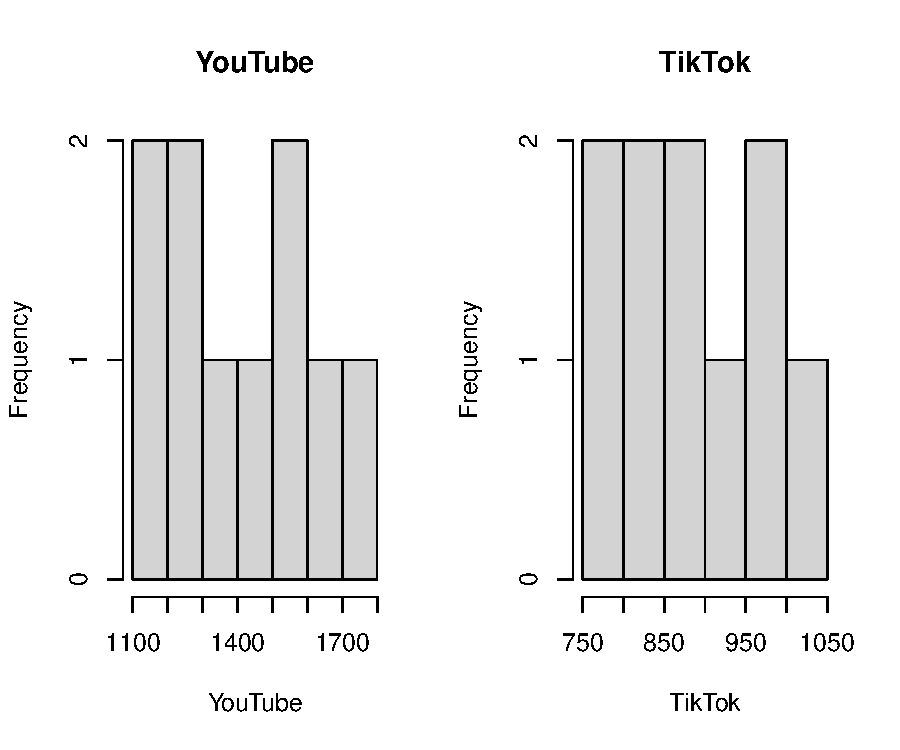
\includegraphics{2_multiple_linear_regression_files/figure-latex/visualization_histogram-1.pdf}
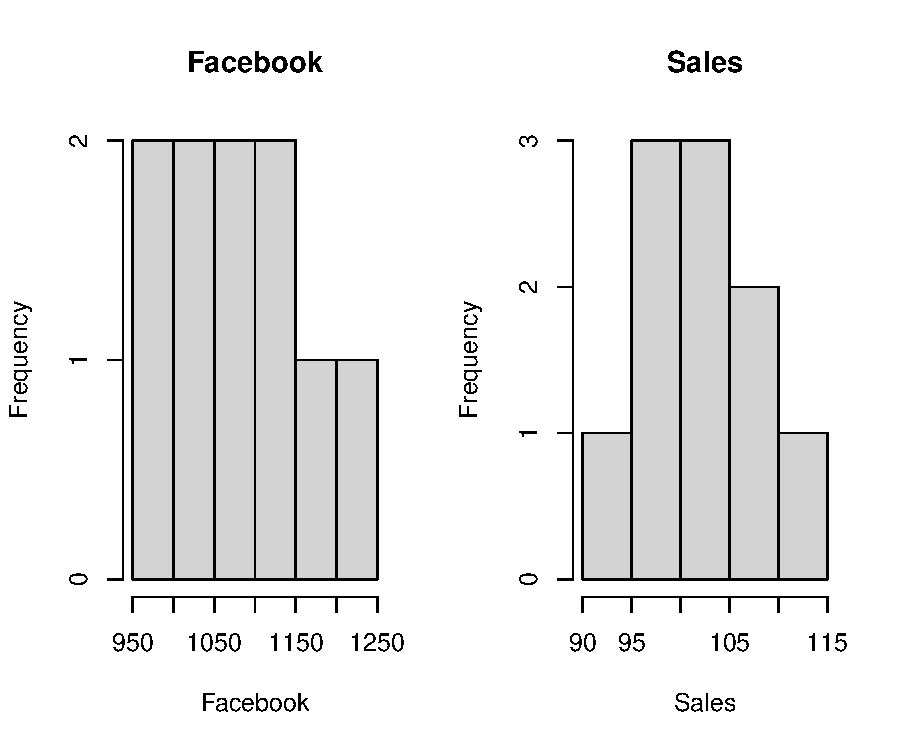
\includegraphics{2_multiple_linear_regression_files/figure-latex/visualization_histogram-2.pdf}

\subsubsection{\texorpdfstring{\textbf{Box and Whisker
Plot}}{Box and Whisker Plot}}\label{box-and-whisker-plot}

\begin{Shaded}
\begin{Highlighting}[]
\CommentTok{\# \textasciigrave{}boxplot()\textasciigrave{} This is the function used to plot the box and whisker plot visualization}
\FunctionTok{par}\NormalTok{(}\AttributeTok{mfrow =} \FunctionTok{c}\NormalTok{(}\DecValTok{1}\NormalTok{, }\DecValTok{2}\NormalTok{))}
\ControlFlowTok{for}\NormalTok{ (i }\ControlFlowTok{in} \DecValTok{1}\SpecialCharTok{:}\DecValTok{4}\NormalTok{) \{}
  \ControlFlowTok{if}\NormalTok{ (}\FunctionTok{is.numeric}\NormalTok{(advertising\_data[[i]])) \{}
    \FunctionTok{boxplot}\NormalTok{(advertising\_data[[i]], }\AttributeTok{main =} \FunctionTok{names}\NormalTok{(advertising\_data)[i])}
\NormalTok{  \} }\ControlFlowTok{else}\NormalTok{ \{}
    \FunctionTok{message}\NormalTok{(}\FunctionTok{paste}\NormalTok{(}\StringTok{"Column"}\NormalTok{, }\FunctionTok{names}\NormalTok{(advertising\_data)[i], }\StringTok{"is not numeric and will be skipped."}\NormalTok{))}
\NormalTok{  \}}
\NormalTok{\}}
\end{Highlighting}
\end{Shaded}

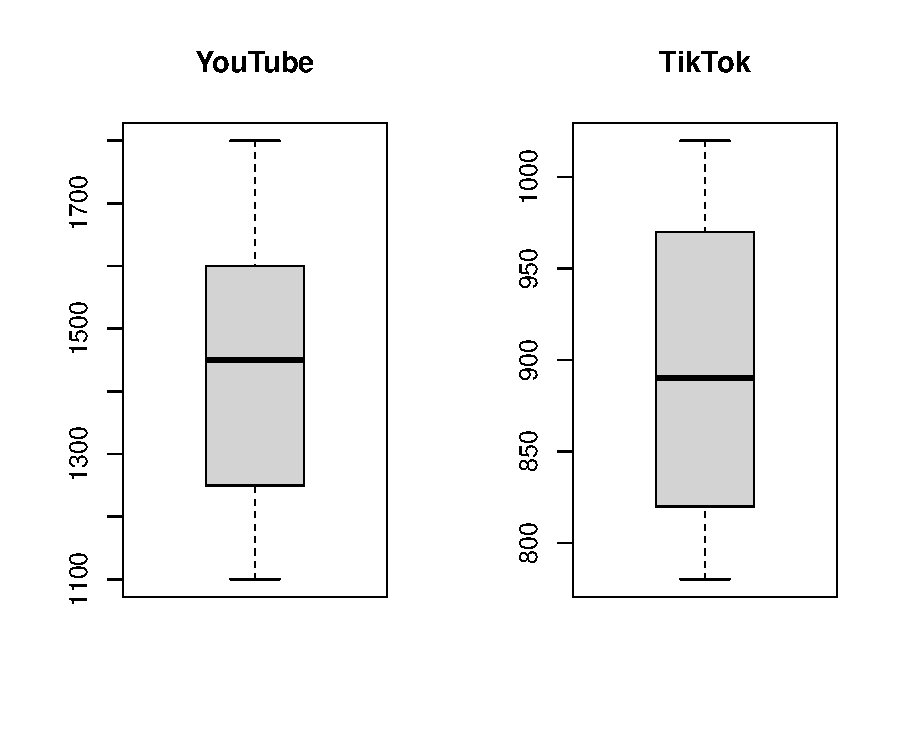
\includegraphics{2_multiple_linear_regression_files/figure-latex/visualization_boxplot-1.pdf}
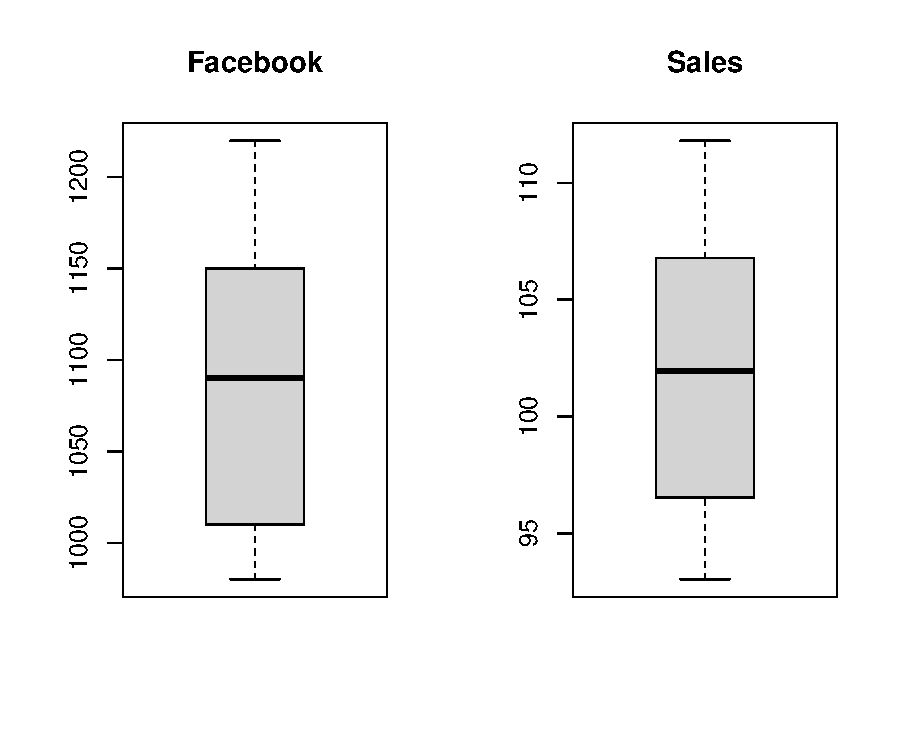
\includegraphics{2_multiple_linear_regression_files/figure-latex/visualization_boxplot-2.pdf}

\subsubsection{\texorpdfstring{\textbf{Missing Data
Plot}}{Missing Data Plot}}\label{missing-data-plot}

\begin{Shaded}
\begin{Highlighting}[]
\NormalTok{pacman}\SpecialCharTok{::}\FunctionTok{p\_load}\NormalTok{(}\StringTok{"Amelia"}\NormalTok{)}

\FunctionTok{missmap}\NormalTok{(advertising\_data, }\AttributeTok{col =} \FunctionTok{c}\NormalTok{(}\StringTok{"red"}\NormalTok{, }\StringTok{"grey"}\NormalTok{), }\AttributeTok{legend =} \ConstantTok{TRUE}\NormalTok{)}
\end{Highlighting}
\end{Shaded}

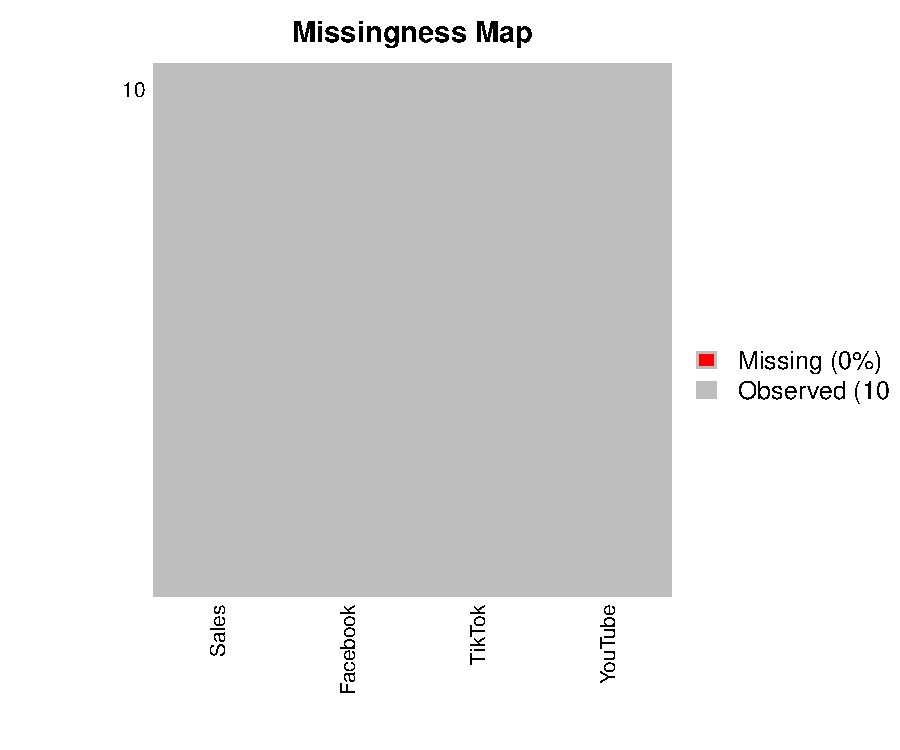
\includegraphics{2_multiple_linear_regression_files/figure-latex/missing_data_plot-1.pdf}

\subsubsection{\texorpdfstring{\textbf{Correlation
Plot}}{Correlation Plot}}\label{correlation-plot}

\begin{Shaded}
\begin{Highlighting}[]
\NormalTok{pacman}\SpecialCharTok{::}\FunctionTok{p\_load}\NormalTok{(}\StringTok{"ggcorrplot"}\NormalTok{)}

\FunctionTok{ggcorrplot}\NormalTok{(}\FunctionTok{cor}\NormalTok{(advertising\_data[,]))}
\end{Highlighting}
\end{Shaded}

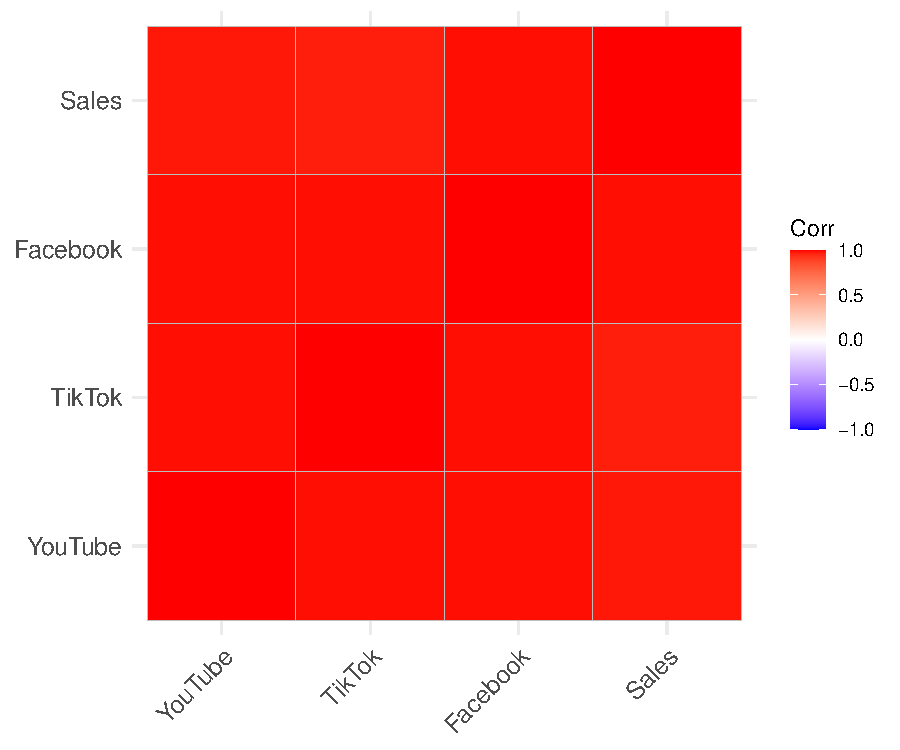
\includegraphics{2_multiple_linear_regression_files/figure-latex/correlation_plot-1.pdf}

\subsubsection{\texorpdfstring{\textbf{Scatter
Plot}}{Scatter Plot}}\label{scatter-plot}

\begin{Shaded}
\begin{Highlighting}[]
\NormalTok{pacman}\SpecialCharTok{::}\FunctionTok{p\_load}\NormalTok{(}\StringTok{"corrplot"}\NormalTok{)}

\FunctionTok{pairs}\NormalTok{(advertising\_data}\SpecialCharTok{$}\NormalTok{Sales }\SpecialCharTok{\textasciitilde{}}\NormalTok{ ., }\AttributeTok{data =}\NormalTok{ advertising\_data, }\AttributeTok{col =}\NormalTok{ advertising\_data}\SpecialCharTok{$}\NormalTok{Sales)}
\end{Highlighting}
\end{Shaded}

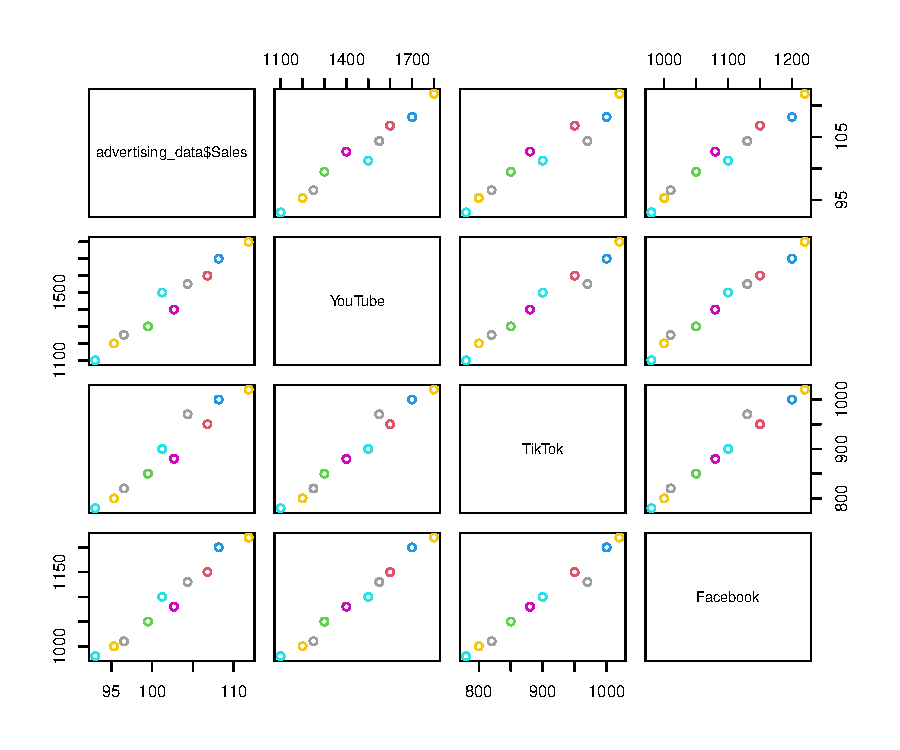
\includegraphics{2_multiple_linear_regression_files/figure-latex/scatter_plot_1-1.pdf}

\begin{Shaded}
\begin{Highlighting}[]
\NormalTok{pacman}\SpecialCharTok{::}\FunctionTok{p\_load}\NormalTok{(}\StringTok{"ggplot2"}\NormalTok{)}
\FunctionTok{ggplot}\NormalTok{(advertising\_data,}
       \FunctionTok{aes}\NormalTok{(}\AttributeTok{x =}\NormalTok{ YouTube, }\AttributeTok{y =}\NormalTok{ Sales)) }\SpecialCharTok{+} 
  \FunctionTok{geom\_point}\NormalTok{() }\SpecialCharTok{+}
  \FunctionTok{geom\_smooth}\NormalTok{(}\AttributeTok{method =}\NormalTok{ lm) }\SpecialCharTok{+}
  \FunctionTok{labs}\NormalTok{(}
    \AttributeTok{title =} \StringTok{"Relationship between Sales Revenue and }\SpecialCharTok{\textbackslash{}n}\StringTok{Expenditure on YouTube Marketing"}\NormalTok{,}
    \AttributeTok{x =} \StringTok{"Expenditure"}\NormalTok{,}
    \AttributeTok{y =} \StringTok{"Sales"}
\NormalTok{  )}
\end{Highlighting}
\end{Shaded}

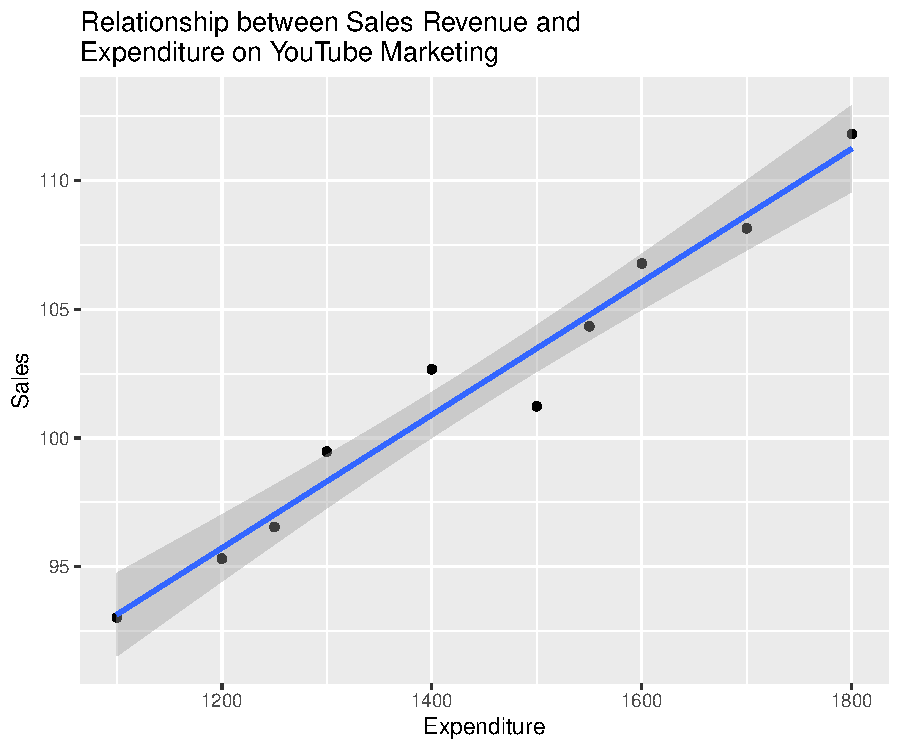
\includegraphics{2_multiple_linear_regression_files/figure-latex/scatter_plot_2-1.pdf}

\begin{Shaded}
\begin{Highlighting}[]
\NormalTok{pacman}\SpecialCharTok{::}\FunctionTok{p\_load}\NormalTok{(}\StringTok{"dplyr"}\NormalTok{)}
\NormalTok{advertising\_data\_composite }\OtherTok{\textless{}{-}}\NormalTok{ advertising\_data }\SpecialCharTok{\%\textgreater{}\%}
  \FunctionTok{mutate}\NormalTok{(}\AttributeTok{Total\_Expenditure =}\NormalTok{ YouTube }\SpecialCharTok{+}\NormalTok{ TikTok }\SpecialCharTok{+}\NormalTok{ Facebook)}

\FunctionTok{ggplot}\NormalTok{(advertising\_data\_composite,}
       \FunctionTok{aes}\NormalTok{(}\AttributeTok{x =}\NormalTok{ Total\_Expenditure, }\AttributeTok{y =}\NormalTok{ Sales)) }\SpecialCharTok{+}
  \FunctionTok{geom\_point}\NormalTok{() }\SpecialCharTok{+}
  \FunctionTok{geom\_smooth}\NormalTok{(}\AttributeTok{method =}\NormalTok{ lm) }\SpecialCharTok{+}
  \FunctionTok{labs}\NormalTok{(}
    \AttributeTok{title =} \StringTok{"Relationship between Sales Revenue and }\SpecialCharTok{\textbackslash{}n}\StringTok{Total Marketing Expenditure"}\NormalTok{,}
    \AttributeTok{x =} \StringTok{"Total Expenditure"}\NormalTok{,}
    \AttributeTok{y =} \StringTok{"Sales"}
\NormalTok{  )}
\end{Highlighting}
\end{Shaded}

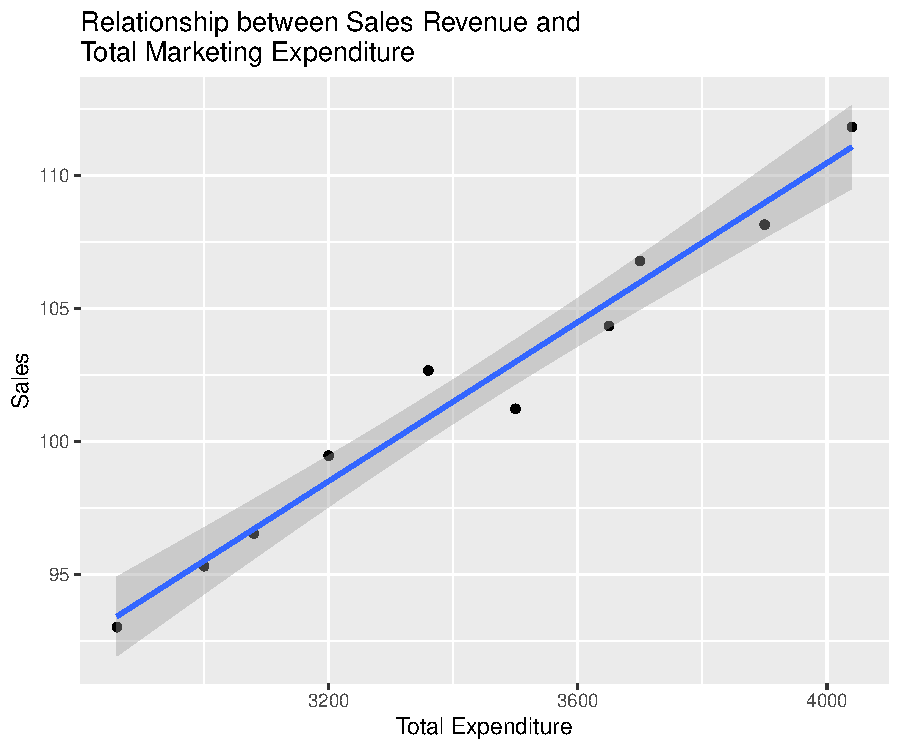
\includegraphics{2_multiple_linear_regression_files/figure-latex/scatter_plot_3-1.pdf}

\section{Statistical Test}\label{statistical-test}

We then apply a simultaneous multiple linear regression as a statistical
test for regression. The term ``simultaneous'' refers to how the
predictor variables are entered and considered in the statistical test.
It means that all the predictor variables included in the model are
entered and evaluated at the same time.

View the summary of the model.

\begin{Shaded}
\begin{Highlighting}[]
\FunctionTok{summary}\NormalTok{(mlr\_test)}
\end{Highlighting}
\end{Shaded}

\begin{verbatim}
## 
## Call:
## lm(formula = Sales ~ YouTube + TikTok + Facebook, data = advertising_data)
## 
## Residuals:
##     Min      1Q  Median      3Q     Max 
## -1.5436 -0.6159  0.1056  0.6598  1.5978 
## 
## Coefficients:
##              Estimate Std. Error t value Pr(>|t|)
## (Intercept) 32.019096  24.432018   1.311    0.238
## YouTube      0.006088   0.015876   0.384    0.715
## TikTok      -0.007662   0.032263  -0.237    0.820
## Facebook     0.062289   0.048787   1.277    0.249
## 
## Residual standard error: 1.2 on 6 degrees of freedom
## Multiple R-squared:  0.9734, Adjusted R-squared:  0.9602 
## F-statistic: 73.32 on 3 and 6 DF,  p-value: 4.055e-05
\end{verbatim}

To obtain a 95\% confidence interval:

\begin{Shaded}
\begin{Highlighting}[]
\FunctionTok{confint}\NormalTok{(mlr\_test, }\AttributeTok{level =} \FloatTok{0.95}\NormalTok{)}
\end{Highlighting}
\end{Shaded}

\begin{verbatim}
##                    2.5 %      97.5 %
## (Intercept) -27.76389745 91.80208927
## YouTube      -0.03275855  0.04493539
## TikTok       -0.08660653  0.07128263
## Facebook     -0.05708823  0.18166580
\end{verbatim}

\section{Diagnostic EDA}\label{diagnostic-eda}

Diagnostic EDA is performed to validate that the regression assumptions
are true with respect to the statistical test. Validating the regression
assumption in turn ensures that the statistical tests applied are
appropriate for the data and helps to prevent incorrect conclusions.

\subsection{\texorpdfstring{\ul{\textbf{Test of
Linearity}}}{Test of Linearity}}\label{test-of-linearity}

The test of linearity is used to assess whether the relationship between
the dependent variables and the independent variables is linear. This is
necessary given that linearity is one of the key assumptions of
statistical tests of regression and verifying it is crucial for ensuring
the validity of the model's estimates and predictions.

A plot of the residuals versus the fitted values enables us to test for
linearity. For the model to pass the test of linearity, there should be
no pattern in the distribution of residuals and the residuals should be
randomly placed around the 0.0 residual line, i.e., the residuals should
randomly vary around the mean of the value of the response variable.

\begin{Shaded}
\begin{Highlighting}[]
\FunctionTok{plot}\NormalTok{(mlr\_test, }\AttributeTok{which =} \DecValTok{1}\NormalTok{)}
\end{Highlighting}
\end{Shaded}

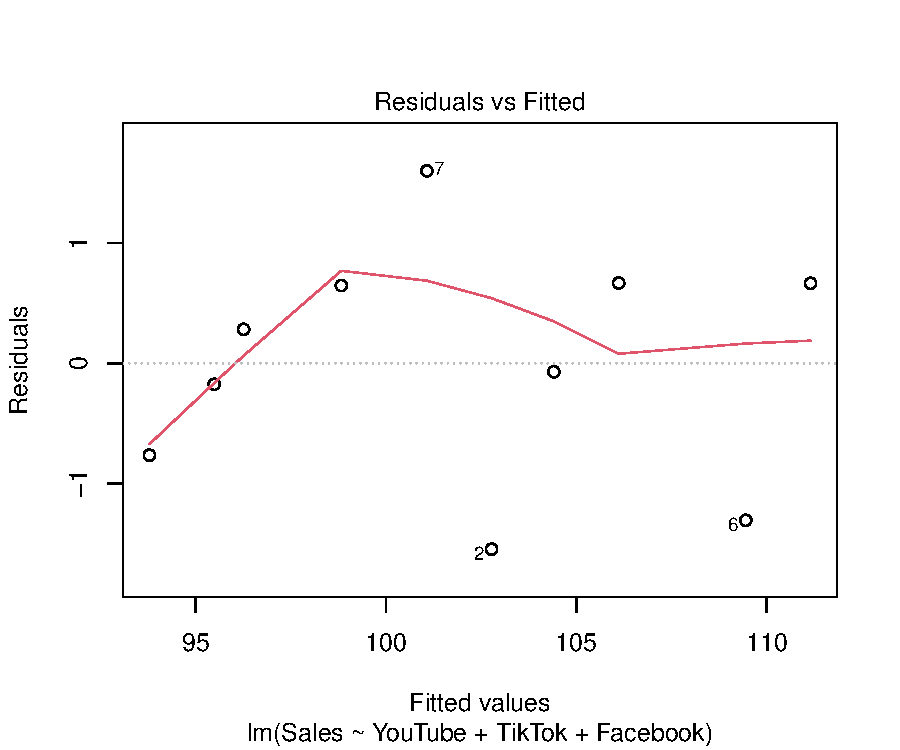
\includegraphics{2_multiple_linear_regression_files/figure-latex/test_of_linearity-1.pdf}

\subsection{\texorpdfstring{\ul{\textbf{Test of Independence of
Errors}}}{Test of Independence of Errors}}\label{test-of-independence-of-errors}

This test is necessary to confirm that each observation is independent
of the other. It helps to identify \textbf{autocorrelation} that is
introduced when the data is collected over a close period of time or
when one observation is related to another observation. Autocorrelation
leads to underestimated standard errors and inflated t-statistics. It
can also make findings appear more significant than they actually are.

The ``\textbf{Durbin-Watson Test}'' can be used as a test of
independence of errors (test of autocorrelation).

\begin{itemize}
\item
  The null hypothesis, H\textsubscript{0}, is that there is no
  autocorrelation
\item
  The alternative hypothesis, H\textsubscript{a}, is that there is
  autocorrelation
\end{itemize}

If the p-value is greater than 0.05 then there is no evidence to reject
the null hypothesis that ``there is no autocorrelation''. The results
below show a p-value of 0.5316, therefore, the test of independence of
errors around the regression line passes.

\begin{Shaded}
\begin{Highlighting}[]
\NormalTok{pacman}\SpecialCharTok{::}\FunctionTok{p\_load}\NormalTok{(}\StringTok{"lmtest"}\NormalTok{)}
\FunctionTok{dwtest}\NormalTok{(mlr\_test)}
\end{Highlighting}
\end{Shaded}

\begin{verbatim}
## 
##  Durbin-Watson test
## 
## data:  mlr_test
## DW = 2.1498, p-value = 0.5316
## alternative hypothesis: true autocorrelation is greater than 0
\end{verbatim}

\subsection{\texorpdfstring{\ul{\textbf{Test of
Normality}}}{Test of Normality}}\label{test-of-normality}

The test of normality assesses whether the residuals are normally
distributed, i.e., most residuals (errors) are close to zero and large
errors are rare. A Q-Q plot can be used to conduct the test of
normality.

A Q-Q plot is a scatterplot of the quantiles of the residuals against
the quantiles of a normal distribution. Quantiles are statistical values
that divide a dataset or probability distribution into equal-sized
intervals. They help in understanding how data is distributed by marking
specific points that separate the data into groups of equal size.
Examples of quantiles include: quartiles (4 equal parts), percentiles
(100 equal parts), deciles (10 equal parts), etc.

If the points in the Q-Q plot fall along a straight line, then the
normality assumption is satisfied. If the points in the Q-Q plot do not
fall along a straight line, then the normality assumption is not
satisfied.

\begin{Shaded}
\begin{Highlighting}[]
\FunctionTok{plot}\NormalTok{(mlr\_test, }\AttributeTok{which =} \DecValTok{2}\NormalTok{)}
\end{Highlighting}
\end{Shaded}

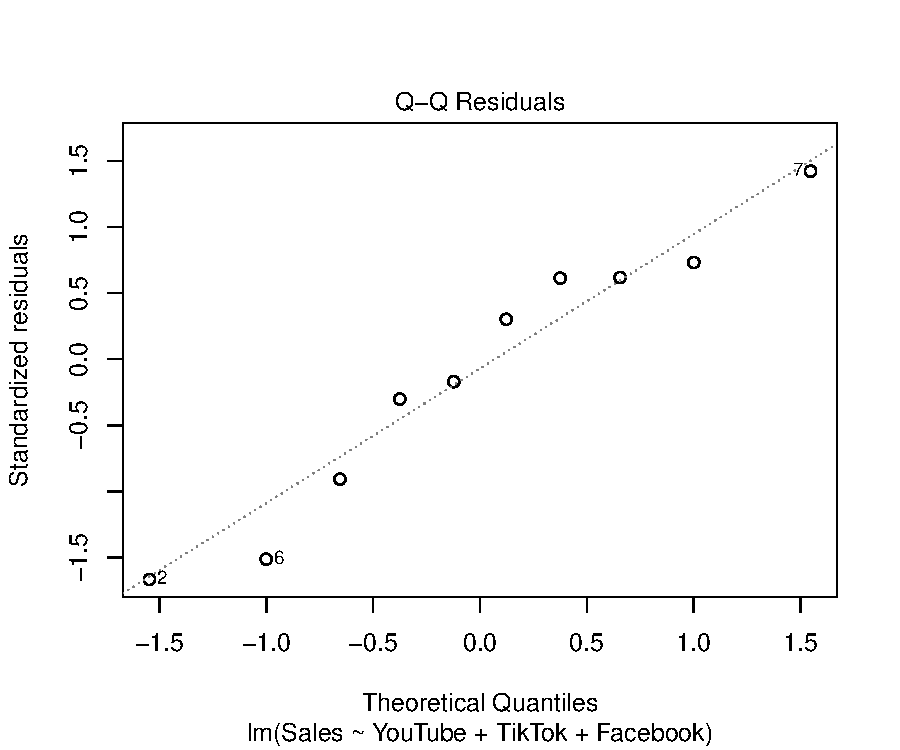
\includegraphics{2_multiple_linear_regression_files/figure-latex/test_of_normality-1.pdf}

\subsection{\texorpdfstring{\ul{\textbf{Test of
Homoscedasticity}}}{Test of Homoscedasticity}}\label{test-of-homoscedasticity}

Homoscedasticity requires that the spread of residuals should be
constant across all levels of the independent variable. A scale-location
plot (a.k.a. spread-location plot) can be used to conduct a test of
homoscedasticity.

The x-axis shows the fitted (predicted) values from the model and the
y-axis shows the square root of the standardized residuals. The red line
is added to help visualize any patterns.

In a model with homoscedastic errors (equal variance across all
predicted values):

\begin{itemize}
\item
  Points should be randomly scattered around a horizontal line
\item
  The smooth line should be approximately horizontal
\item
  The vertical spread of points should be roughly equal across all
  fitted values
\item
  No obvious patterns, funnels, or trends should be visible
\end{itemize}

Points forming a cone shape that widens from left to right suggests
heteroscedasticity with increasing variance for larger fitted values.

\begin{Shaded}
\begin{Highlighting}[]
\FunctionTok{plot}\NormalTok{(mlr\_test, }\AttributeTok{which =} \DecValTok{3}\NormalTok{)}
\end{Highlighting}
\end{Shaded}

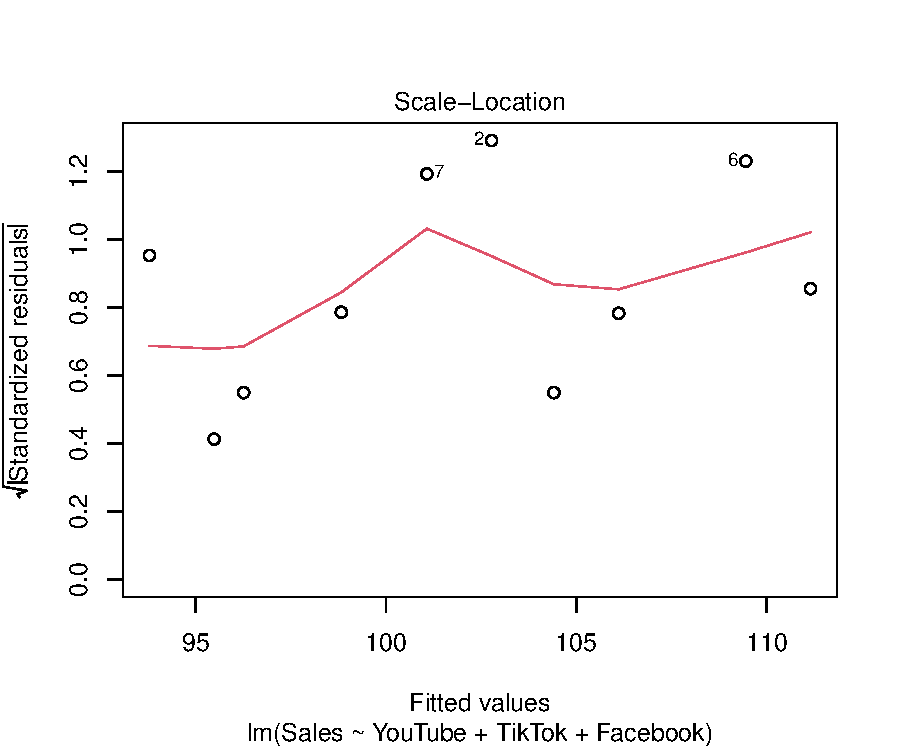
\includegraphics{2_multiple_linear_regression_files/figure-latex/test_of_homoscedasticity-1.pdf}

\subsection{\texorpdfstring{\ul{\textbf{Quantitative Validation of
Assumptions}}}{Quantitative Validation of Assumptions}}\label{quantitative-validation-of-assumptions}

The graphical representations of the various tests of assumptions should
be accompanied by quantitative values. The \texttt{gvlma} package
(Global Validation of Linear Models Assumptions) is useful for this
purpose.

\begin{Shaded}
\begin{Highlighting}[]
\NormalTok{pacman}\SpecialCharTok{::}\FunctionTok{p\_load}\NormalTok{(}\StringTok{"gvlma"}\NormalTok{)}
\NormalTok{gvlma\_results }\OtherTok{\textless{}{-}} \FunctionTok{gvlma}\NormalTok{(mlr\_test)}
\FunctionTok{summary}\NormalTok{(gvlma\_results)}
\end{Highlighting}
\end{Shaded}

\begin{verbatim}
## 
## Call:
## lm(formula = Sales ~ YouTube + TikTok + Facebook, data = advertising_data)
## 
## Residuals:
##     Min      1Q  Median      3Q     Max 
## -1.5436 -0.6159  0.1056  0.6598  1.5978 
## 
## Coefficients:
##              Estimate Std. Error t value Pr(>|t|)
## (Intercept) 32.019096  24.432018   1.311    0.238
## YouTube      0.006088   0.015876   0.384    0.715
## TikTok      -0.007662   0.032263  -0.237    0.820
## Facebook     0.062289   0.048787   1.277    0.249
## 
## Residual standard error: 1.2 on 6 degrees of freedom
## Multiple R-squared:  0.9734, Adjusted R-squared:  0.9602 
## F-statistic: 73.32 on 3 and 6 DF,  p-value: 4.055e-05
## 
## 
## ASSESSMENT OF THE LINEAR MODEL ASSUMPTIONS
## USING THE GLOBAL TEST ON 4 DEGREES-OF-FREEDOM:
## Level of Significance =  0.05 
## 
## Call:
##  gvlma(x = mlr_test) 
## 
##                      Value p-value                Decision
## Global Stat        0.92304  0.9212 Assumptions acceptable.
## Skewness           0.04975  0.8235 Assumptions acceptable.
## Kurtosis           0.30420  0.5813 Assumptions acceptable.
## Link Function      0.41234  0.5208 Assumptions acceptable.
## Heteroscedasticity 0.15675  0.6922 Assumptions acceptable.
\end{verbatim}

\subsection{Test of Multicollinearity}\label{test-of-multicollinearity}

Multicollinearity arises when two or more independent variables
(predictors) are highly intercorrelated. The \textbf{Variance Inflation
Factor (VIF)} quantifies how much the variance of a coefficient estimate
is ``inflated'' due to multicollinearity. A VIF of 1 indicates no
collinearity; values above 5 suggest problematic levels of collinearity.
High VIF values (VIF \textgreater{} 5) suggest that the coefficient
estimates are less reliable due to the correlations between predictors.

\begin{Shaded}
\begin{Highlighting}[]
\NormalTok{pacman}\SpecialCharTok{::}\FunctionTok{p\_load}\NormalTok{(}\StringTok{"car"}\NormalTok{)}
\FunctionTok{vif}\NormalTok{(mlr\_test)}
\end{Highlighting}
\end{Shaded}

\begin{verbatim}
##   YouTube    TikTok  Facebook 
##  82.13782  47.30912 103.46518
\end{verbatim}

\section{Interpretation of the
Results}\label{interpretation-of-the-results}

\subsection{Academic Statement}\label{academic-statement}

A simultaneous multiple linear regression analysis was conducted on data
from 10 observations (N=10) to examine whether advertising expenditures
on YouTube, TikTok, and Facebook collectively predict Sales. The results
indicated that neither expenses on YouTube (\(\beta\) = 0.01, 95\% CI
{[}-.03, .04{]}, SE = 0.02, \emph{t}(6) = 0.38, \emph{p} = .715), nor
TikTok (\(\beta\) = -0.01, 95\% CI {[}-.09, .07{]}, SE = 0.03,
\emph{t}(6) = -0.24, \emph{p} = .820) nor Facebook (\(\beta\) = 0.06,
95\% CI {[}-.06, .18{]}, SE = 0.05, \emph{t}(6) = 1.28, \emph{p} = .249)
individually significantly predicted Sales (all \emph{p} \textgreater{}
0.05). The model explained 97.34\% of the variance in Sales (Multiple
R\textsuperscript{2} = .97, Adjusted R\textsuperscript{2} = .96,
\emph{F}(3, 6) = 73.32, \emph{p} \textless{} .001). The intercept was
32.02, 95\% CI {[}-27.76, 91.80{]}, SE = 24.43, \emph{t}(6) = 1.31,
\emph{p} = .238. The residual standard error was 1.2, indicating a
robust model. The full results are presented in the table below.

\begin{longtable}[]{@{}cccccc@{}}
\caption{Regression Coefficients Predicting Sales from Multiple
Advertising Channels}\tabularnewline
\toprule\noalign{}
Predictor & \(\beta\) & 95\% CI & SE & \emph{t}(6) & \emph{p} \\
\midrule\noalign{}
\endfirsthead
\toprule\noalign{}
Predictor & \(\beta\) & 95\% CI & SE & \emph{t}(6) & \emph{p} \\
\midrule\noalign{}
\endhead
\bottomrule\noalign{}
\endlastfoot
(Intercept) & 32.02 & {[}-27.76, 91.80{]} & 24.43 & 1.31 & .238 \\
YouTube & 0.01 & {[}-.03, .04{]} & 0.02 & 0.38 & .715 \\
TikTok & -0.01 & {[}-.09, .07{]} & 0.03 & -0.24 & .820 \\
Facebook & 0.06 & {[}-.06, .18{]} & 0.05 & 1.28 & .249 \\
\end{longtable}

\textbf{\emph{Note.}} N\,=\,10; SE\,=\,standard error; CI\,=\,confidence
interval.

Even though the results indicated a robust model whereby advertisement
expenditures collectively predict sales, individual parameter estimates
did not reach statistical significance when controlling for the other
parameters. This suggests that the advertising channels collectively
explain variation in Sales but do not uniquely predict Sales in this
small sample. This may reflect multicollinearity among the different
advertising platforms or limited statistical power due to the small
sample size (\emph{N} = 10). Future research should investigate these
predictors with a larger sample and assess potential collinearity.

\subsection{Business Analysis}\label{business-analysis}

Although aggregate digital advertising spend across YouTube, TikTok, and
Facebook is highly predictive of Sales (accounting for nearly all
observed variation), the absence of statistically significant individual
coefficients indicates that no single channel can be reliably credited
with driving incremental Sales in this dataset. This finding suggests
that, within the current investment levels and the constraints of a
small sample, the three platforms function as a cohesive portfolio
rather than as independent drivers of sales revenue. Recommendation for
management:

\begin{enumerate}
\def\labelenumi{\arabic{enumi}.}
\tightlist
\item
  Continue to view YouTube, TikTok, and Facebook as complementary
  elements of a unified digital marketing strategy focusing on the total
  expenditure rather than favouring a single platform.
\end{enumerate}

\subsection{Limitations}\label{limitations}

\begin{enumerate}
\def\labelenumi{\arabic{enumi}.}
\item
  Small Sample Size (N\,=\,10): Using a limited number of observations
  restricts statistical power and inflates standard errors, raising the
  risk of a Type II error (failing to detect true channel effects).
\item
  Potential Multicollinearity: High intercorrelations among YouTube,
  TikTok, and Facebook expenditures may obscure unique contributions.
\item
  Restricted Expenditure Range: Limited range of advertisement
  expenditures impairs the ability to detect linear effects.
\item
  Methodology: Lack of experimental variation in advertisement
  expenditure limits causal attribution to any single platform.
\end{enumerate}

\end{document}
